\documentclass{beamer}
\usepackage{amsthm}

\usetheme{Berkeley}
\usecolortheme{seahorse}

\title{Metodos matemáticos para la computación cuántica}
\subtitle{Tensores}
\author{Santiago Klepp}
\date{19 de Mayo de 2026}

\newtheorem{teo}{Teorema}
\newtheorem{defi}{Definición}
\newtheorem{ejemplo}{Ejemplo}

\begin{document}

\frame{\titlepage}

\section{Matemática}
\subsection{Algebra Lineal}
\begin{frame}
\frametitle{Producto interno}
\begin{defi}
Un \textbf{producto interno} del espacio vectorial $V$ al cuerpo $F$
    es una función  $( \cdot,\cdot ) : V \times V \to F$ tal que
para $x,y \in V, a,b \in F$:
\begin{itemize}
    \item $( x,y ) = \overline{( y,x )}$ donde $\overline{\cdots}$ es el conjugado en el espacio $F$.
    \item $( ax + by,z ) = a ( x,z ) + b ( y,z )$
    \item $( x,x ) > 0 \iff x \neq 0$
\end{itemize}
\end{defi}

\pause
\begin{ejemplo}
Si $x, y \in F^n$, entonces
$$
    ( x,y ) = \sum_{k=1}^n x_k\overline{y_k}
$$
es un producto interno
\end{ejemplo}

\end{frame}
\begin{frame}
\frametitle{Producto interno}
\begin{ejemplo}
Si $V$ es el espacio de funciones contínuas en $[a,b]$, entonces
tomando $f,g \in V$ se tiene que 
$$
    ( f,g ) = \int_a^b f(x) g(x) dx 
$$
es un producto interno
\end{ejemplo}
\pause

\begin{defi}
    Un espacio vectorial $V$ con un producto interno $( \cdot,\cdot )$ es un \textbf{espacio con producto interno}.
\end{defi}

\end{frame}

\begin{frame}
    \frametitle{Producto interno}
    \begin{teo}
        Si $u, v \in V$ con $V$ un espacio vectorial, sea $u = [u_1,\cdots,u_n], v = [v_1,\cdots, v_n]$ la representación
        vectorial de $u,v$. Entonces:
        $$
        (u,v) = u^T v
        $$
        donde $A^T$ es la transpuesta de $A$
    \end{teo}
\end{frame}

\begin{frame}
\frametitle{Norma}
\begin{defi}
Sea $X$ es un espacio vectorial sobre un cuerpo $F$. Una \textbf{norma} en $X$
es una función dada por $|| \cdot || : X \to F$ que verifica $\forall x,y \in V, c \in F$:
\begin{itemize}
\item $||x|| \geq 0$
\item $||x|| = 0 \iff x = 0$
\item $||c x|| = |c| ||x||$
\item $||x + y|| \leq ||x|| + ||y||$
\end{itemize}
\end{defi}
\pause

    \begin{ejemplo}[Norma inducida por producto interno]
        La función dada por $|| \cdot || = \sqrt{( \cdot, \cdot )}$ con $( \cdot, \cdot )$
        un producto interno en $X$ es una norma en $X$. Esta norma
        se llama norma inducida por producto interno.
    \end{ejemplo}
\end{frame}

\begin{frame}
\frametitle{Norma}
\begin{ejemplo}
La distancia euclideana en $\mathbb{R}^n$ dada por
$$
||x|| = \sqrt{\sum_{k=1}^n x_k^2}
$$
es una norma en $\mathbb{R}^n$.

\end{ejemplo}
\pause

\begin{ejemplo}[$L_p$]
Mas generalmente, la norma $L_p$ dada por
$$
||x||_p = (\sum_{k=1}^n |x_k|^p)^{\frac{1}{p}}
$$
es una norma en $\mathbb{R}^n$.
\end{ejemplo}

\end{frame}

\begin{frame}
\begin{defi}
\frametitle{Espacio Normado}
Un espacio vectorial $V$ equipado de una norma $||\cdot||$ es un \textbf{espacio normado}.
\end{defi}
\pause

\begin{teo}
    Sea $V$ un espacio con producto interno, entonces la función $|| \cdot || = \sqrt{( \cdot,\cdot )}$
    define una norma en $V$ y $V$ es un espacio normado.
\end{teo}
\pause

En conclusión:

    Espacio con producto interno $\implies$ Espacio normado

\end{frame}


\begin{frame}
\frametitle{Funcionales lineales}
\begin{defi}
Un \textbf{funcional lineal} es una transformación lineal de $V$ a $F$ donde
$V$ es un espacio vectorial y $F$ es el cuerpo en el cual está definida la transformación
\end{defi}

\pause
\begin{ejemplo}
Si $V$ es el espacio de funciones contínuas reales en $[0,2\pi]$ y $g \in V$, entonces
$h:V -> \mathbb{R}$ dada por

$$
h(x) = \frac{1}{2\pi} \int_0^{2\pi} x(t)g(x) dt
$$
es una transformación lineal (recordar que el $x$ de $h(x)$ es una función de valores reales)

\end{ejemplo}

\end{frame}

\begin{frame}
    \frametitle{Espacio dual}
    \begin{defi}
        El espacio vectorial de todas las transformaciones lineales de $V$ a $W$ se denota por $\mathcal{L}(V;W)$.
    \end{defi}
\pause
    \begin{defi}
        Para un espacio vectorial $V$ sobre $F$, el \textbf{espacio dual} $V^*$ de $V$ es el espacio
        vectorial de todos los funcionales de $V$ a $F$, o sea $\mathcal{L}(V;F).$
    \end{defi}
\pause
    \begin{defi}
        Se denomina función \textbf{Dirac-Delta} a la función
        $$
        \delta_{ij}=
            \begin{cases}
             1& \text{si } i=j\\
             0& \text{si } i \neq j.
            \end{cases}
        $$
    \end{defi}
\end{frame}

\begin{frame}
    \frametitle{Espacio dual}
    Que forma tiene el espacio dual?
    \begin{teo}
        Sea $V$ es un espacio vectorial de dimensión finita con base ordenada $\beta = {x_1,...,x_n}$.
        Sea $f_i$ dada por $f_i(x_j) = \delta_{ij}$. Entonces $\beta^* = {f_1,...,f_n}$ es una 
        base ordenada para $V^*$ y cada elemento $f \in V^*$ se tiene que.
        $$
        f = \sum_{i=1}^n f(x_i)f_i
        $$
    \end{teo}
\pause
    \begin{defi}
        La base descrita en el teorema anterior se dice que es la \textbf{base dual} de $\beta$.
    \end{defi}
\end{frame}

\begin{frame}
    La base dual nos permite rescatar la coordenada que querramos en la base ordenada que tenga $V$.
\end{frame}

\begin{frame}
    \frametitle{Doble dual}
    \begin{defi}
        Se dice que dos espacios $V$ y $W$ son isomorfos si existe una función lineal $f$ que sea 1 a 1.
        A esta relación se la denota como $V \cong W$.
    \end{defi}
\pause
    \begin{defi}
        El doble dual $V^{**}$ está definido como
        $$
        V^{**} = (V^*)^*
        $$
        osea, el dual del dual de $V$.
    \end{defi}
\end{frame}

\begin{frame}
    \frametitle{Doble dual}
    \begin{teo}
        Si $V$ es un espacio vectorial de dimensión finita, entonces:
        $$V \cong V^{**}$$
    \end{teo}
\pause
    \begin{teo}
        Sea $V$ es un espacio vectorial de dimensión finita con espacio dual $V^*$.
        Entonces toda base ordenada de $V^*$ es el dual para una base de $V$.
    \end{teo}
\pause

    La demostración usa el hecho de que $V \cong V^{**}$. Esto nos garantiza que $V$ puede ser reconstruido
    conociendo sus funcionales en $V^*$.
\end{frame}

%\begin{frame}
    %\frametitle{Notación de Einstein}
%
%\end{frame}

\begin{frame}
    \frametitle{Funciones multilineales}
    \begin{defi}
        Una \textbf{función multilineal} es una función $f$ tal que $f: V_1 \times ... \times V_n \to W$ donde
        $$
        f(x_1,...,x_k+\lambda y,...,x_n) = f(x_1,...,x_k,...,x_n) + \lambda f(x_1,...,y,...,x_n)
        $$
    \end{defi}
\pause
    O sea, una función multilineal es lineal en sus coordenadas.
    
\end{frame}

\begin{frame}
    \frametitle{Funciones multilineales}
    \begin{ejemplo}
        El determinante es una función multilineal porque
        $$
        \begin{aligned}
\begin{vmatrix}
v_1 & \cdots & v_i+\mu w & \cdots & v_n
\end{vmatrix}
&=
\begin{vmatrix}
v_1 & \cdots & v_i & \cdots & v_n
\end{vmatrix}
\\[1ex]
&\quad+
\mu
\begin{vmatrix}
v_1 & \cdots & w & \cdots & v_n
\end{vmatrix}
\end{aligned}
        $$
        donde $v_1,\cdots,v_n,w \in V$ y $\mu \in F$.
    \end{ejemplo}
\pause
    Dato de color. Las funciones multilineales forman un espacio vectorial de funciones que van de
    $V_1\times ...\times V_n$ a $W$ y se ese espacio se denota por $\mathcal{L} (V_1,...,V_n ;W)$.
\end{frame}


\begin{frame}
    \frametitle{Lo que todos estábamos esperando}
    
\includegraphics{esperando.jpg}
\end{frame}

\subsection{Tensores}
\begin{frame}
    \frametitle{Tensores}
    Tensores!!!!

    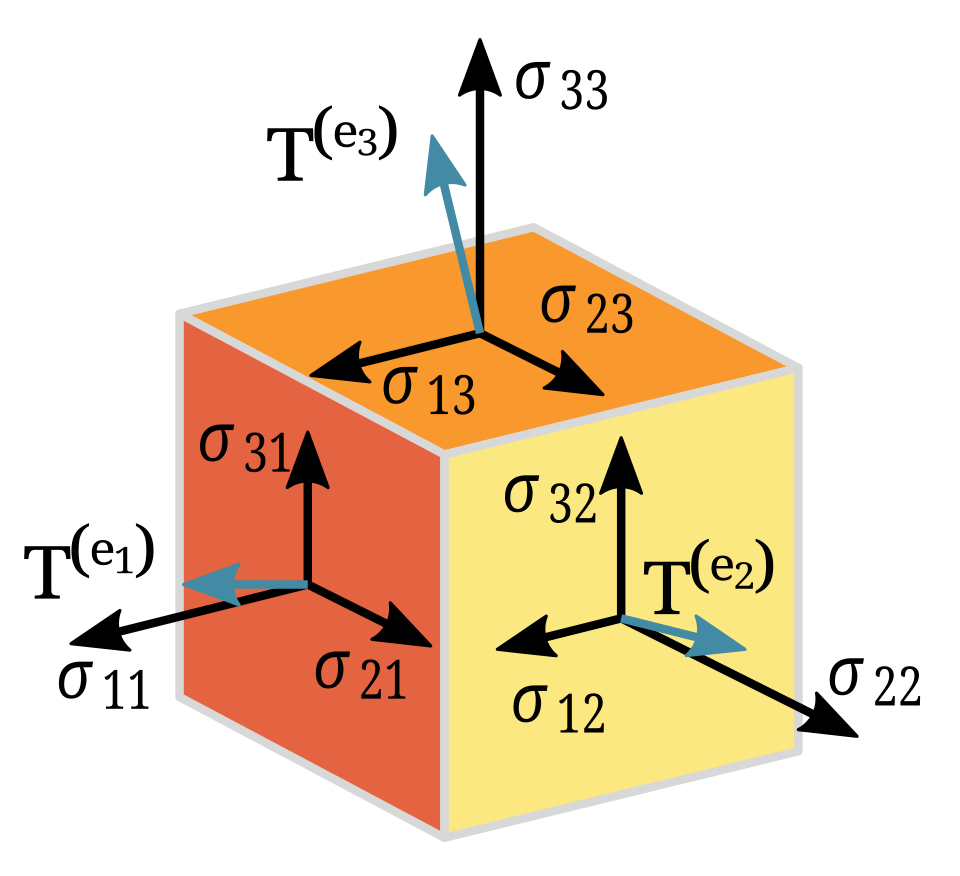
\includegraphics[height=5cm]{tensores.png}
    
\end{frame}

\begin{frame}
    \frametitle{Producto tensorial}
    \begin{defi}
        Un \textbf{producto tensorial} de \underline{espacios vectoriales} $V_1,...,V_n$ denotado como
        $V_1 \otimes ... \otimes V_n$ es un espacio vectorial con un mapa
        $$
        \otimes : V_1 \times ... \times V_n \to V_1 \otimes ... \otimes V_n
        $$
        donde
        \begin{itemize}
            \item $\otimes$ es multilineal 
            \item (propiedad universal) si hay un mapa $f : V_1 \times ... \times V_n \to Y$,
                entonces existe un único mapa lineal
                $$
                \hat{f} : V_1 \otimes ... \otimes V_n \to Y
                $$
                tal que $f = \hat{f} \circ \otimes$.
        \end{itemize}
    \end{defi}
\end{frame}

\begin{frame}
    \frametitle{Producto tensorial}
    \begin{teo}
        $$
        V_1 \otimes ... \otimes V_n \cong \mathcal{L}(V_1^*,...,V_n^*;F)
        $$
    \end{teo}
    \pause
    \begin{teo}
        El producto tensorial de $V_1,...,V_n$ siempre existe y cualquier
        producto tensorial de $V_1,...,V_n$ es isomorfo entre si.
    \end{teo}
\end{frame}


\begin{frame}
    \frametitle{Tensores}
    La gracia de definir este espacio es que garantiza que cualquier mapa multilineal
    $V_1 \times ... \times V_n$ factorize de forma única en un mapa lineal definido
    en el producto tensorial compuesto por un elemento del espacio producto tensorial.
\end{frame}

\begin{frame}
    \frametitle{Tensores}
    Las propiedades algebráicas heredadas de la definición son:
    \begin{itemize}
        \item $$
            \begin{aligned}
                &x_1 \otimes ... \otimes (x_i + x_i') \otimes ... \otimes x_n =\\
                &(x_1 \otimes ... \otimes x_i \otimes ... \otimes x_n) + (x_1 \otimes ... \otimes x_i' \otimes ... \otimes x_n)
            \end{aligned}
            $$
        \item $$
            \begin{aligned}
                (a x_1) \otimes ... \otimes x_j ...\otimes x_n &=x_1 \otimes ... \otimes (a x_j) ...\otimes x_n \\
                &=a(x_1 \otimes ... \otimes x_j ...\otimes x_n) : a \in F
            \end{aligned}
            $$
    \end{itemize}
\end{frame}

\begin{frame}
    \frametitle{Tensores}
    Los elementos típicos del espacio del producto tensorial son:
    \begin{itemize}
        \item simples: $x_1\otimes ... \otimes x_n$ con $x_k \in V_k$
        \item compuestos: $\sum_{i=1}^n x_{i1}\otimes ... \otimes x_{in}$ con $x_{kj} \in V_k : j \in [1,n]$
    \end{itemize}
\end{frame}

\begin{frame}
    \frametitle{Tensores}
    \begin{ejemplo}
        $$
        \begin{aligned}
            x \otimes y + x' \otimes y' &= ( \frac{1}{2} x + \frac{1}{2} x') \otimes (y + y')\\
            &+ ((x+x')\otimes (y+y')) \frac{1}{2}
        \end{aligned}
        $$
    \end{ejemplo}
\end{frame}

\begin{frame}
    \frametitle{Isomorfismo con matrices}
    \begin{teo}[Isomorfismo tensorial]
        $$
        V_1^* \otimes ... \otimes V_n^* \cong (V_1 \otimes ... \otimes V_n)^*
        $$
    \end{teo}
    \pause
	\begin{teo}
		Sean $X, Y$ dos espacios vectoriales. Entonces
		$$
		\mathcal{L} (X;Y) \cong X^* \otimes Y.
		$$
	\end{teo}
    \pause
    Estos 2 teoremas permiten identificar un producto tensorial con un elemento 
    del espacio de $\mathcal{L}(X,Y)$ (una matriz).

\end{frame}

\begin{frame}
    \frametitle{(p,q)-Tensores}
    \begin{defi}
        \[
        V_p^q = \underbrace{
        V^* \otimes \cdots \otimes V^*
        }_{p\text{ veces}}
        \otimes
        \underbrace{
        V \otimes \cdots \otimes V
        }_{q\text{ veces}}
        \]
    \end{defi}
    \pause
    \begin{defi}
        \[
            \mathcal{L}(\underbrace{
        V^* \otimes \cdots \otimes V^*
        }_{p\text{ veces}}
        \otimes
        \underbrace{
        V \otimes \cdots \otimes V
    }_{q\text{ veces}}; F)
        \]

        denotado como $V_p^q$ es el \textbf{espacio de $(p,q)$-tensores}
        y un elemento de este espacio es un \textbf{tensor}.
    \end{defi}
\end{frame}
\begin{frame}
    \begin{ejemplo}
        Si $T$ es un tensor, entonces por el teorema del isomorfismo tensorial
        se puede ver que tiene la forma de
        $$
        T : V_1^* \times ... \times V_p^* \times V_1 \times ... \times V_q \to F
        $$
    \end{ejemplo}
\end{frame}

\begin{frame}
    \frametitle{(p,q)-Tensores NOTACIÓN}

	Los espacios tensoriales pueden tener estas formas
	$$
	X \otimes X\otimes X\otimes X^* \otimes X\otimes X^* \otimes X^*
	$$
	\pause
	Este espacio se denota como $X^3{_1}^1{_2}$ (obviamente isomorfo a $X_3^4$).
    \pause

    Esta clase de espacios donde los tensores junto a los duales no están agrupados
    por cada tipo se les dice \textbf{mixtos}.
\end{frame}


\begin{frame}
	\frametitle{Producto tensorial entre mapas}
	\begin{teo}
		Si $A_i : X_i \to Y_i$ son funciones lineales, entonces
		$$
		X_1 \times ... \times X_n \to_{A_1,...,A_n} Y_1 \times ... \times Y_n \to_{\otimes} Y_1 \otimes ... \otimes Y_n
		$$
		es multilineal. La forma de este mapa es:
		$$
		(x_1,...,x_n) \mapsto (A_1 x_1 ,... , A_n x_n) \mapsto (A_1 x_1 \otimes ... \otimes A_n x_n)
		$$
	\end{teo}
\end{frame}

\begin{frame}
	\frametitle{Contracciones}
	\begin{defi}
		Para cualquier espacio producto (p,q)-tensorial, se define la contracción
		$$
		\mathcal{C}_i^j : V_p^q \to V_{p-1}^{q-1}
		$$
		Dada por
		$$
		\begin{aligned}
			&\mathcal{C}_i^j(x_1\otimes ...\otimes x_p\otimes x^1 \otimes ...\otimes x^q)\\
			&= (x_1\otimes...\otimes \hat{x_{i}} \otimes ...\otimes x_{p}\otimes x^1 \otimes ... \otimes \hat{x^{j}} \otimes ...\otimes x^p) (x_i(x^j))
		\end{aligned}
		$$
	\end{defi}
	\pause
    La contracción también está definida sobre un producto mixto ya que 
    esos espacios son isomorfos a uno de la forma $V_i^j$.
\end{frame}

\begin{frame}
	\frametitle{Producto tensorial entre dos tensores}
	Si $u \in V_i^j$ y $v \in V_k^l$, entonces
	$u \otimes v \in V_i{^j}{_k}^l \cong V_{i+k}^{j+l}$
\end{frame}

\begin{frame}
	\frametitle{Producto de Kronecker}
	Sea $V,W,Y,Z$ espacios vectoriales con bases dadas.
	\pause
	Sean $S: V\to Y$ y $T: W\to Z$ son funciones lineales y $A, B$ sus representaciones matriciales.
	\pause
	\begin{defi}
		$$
		A \otimes B = 
		\begin{bmatrix}
		a_{11}B & \cdots & a_{1n}B \\
		\vdots & \ddots & \vdots \\
		a_{m1}B & \cdots & a_{mn}B
		\end{bmatrix}
		$$
		donde
		$$
		a_{ij} B = 
		\begin{bmatrix}
			a_{ij} b_{11} & \cdots & a_{ij} b_{1n} \\
		\vdots & \ddots & \vdots \\
			a_{ij} b_{m1} & \cdots & a_{ij} b_{mn}
		\end{bmatrix}
		$$
	\end{defi}
\end{frame}

\begin{frame}
	\frametitle{Producto de Kronecker - Propiedades}
	Son las del producto tensorial.
	\begin{itemize}
		\item $A \otimes (B + C) = A \otimes B + A\otimes C$
		\item $(B+C) \otimes A = (B\otimes A) + (C\otimes A)$
		\item $(k A) \otimes B = A \otimes (k B) = k A \otimes B$
		\item $(A \otimes B) \otimes C = A \otimes (B \otimes C)$
	\end{itemize}
	\pause
	NO es conmutativa.
\end{frame}

\begin{frame}
	\frametitle{Producto de Kronecker - Propiedades}
	Por la propiedad de los productos tensoriales entre mapas se tiene que
	$$
	(A \otimes B) (C \otimes D) = (AC) \otimes (BD)
	$$
\end{frame}


\subsection{Espacios de Hilbert}
\begin{frame}
    \frametitle{Espacio métrico}
    \begin{defi}
        Una \textbf{métrica} en un conjunto $M$ es una función $d : M \times M \to \mathbb{R}$ tal que
        \begin{itemize}
            \item $d(x,y) \geq 0$
            \item $d(x,y) = 0 \iff x = y$
            \item $d(x,y) = d(y,x)$
            \item $d(x,z) \leq d(x,y) + d(y,z)$
        \end{itemize}
    \end{defi}
	\pause
    \begin{defi}
        El par ordenado $(M,d)$ donde $M$ es un conjunto y $d$ es una métrica en $M$ se dice \textbf{espacio métrico}.
    \end{defi}
\end{frame}

%TODO: hablar del producto de kronecker y cerrar tensores

%En cuántica hablar de la definición de qubit. Su representación explícita de blosch
%quantum gates y registros cuánticos y como los registros son tensores y justamente isomorfos a una matriz

% Cerrar con el algoritmo de Deutsch


\begin{frame}
\frametitle{Espacio métrico}
    \begin{teo}
        Sea $X$ es un espacio vectorial con norma $|| \cdot ||$. Si $d: X \times X \to F$ dada por
        $d(x,y) = ||y-x||$, entonces $(X,d)$ es un espacio métrico.
    \end{teo}
	\pause
    En conclusión:

    Espacio normado $\implies$ Espacio métrico.
	\pause
    \begin{defi}
        La distancia $d(x,y) = ||y-x||$ se llama distancia inducida por la norma de $X$.
    \end{defi}
\end{frame}

\begin{frame}
\frametitle{Espacio métrico completo}
    \begin{defi}
        Una secuencia es de \textbf{Cauchy} si $forall epsilon >0$, existe $N \in \mathbb{N}$ tal que
        $$
        d(x_m,x_n) < \epsilon\;\;\; \forall m,n \geq N
        $$
    \end{defi}
	\pause
\begin{defi}
    Un espacio métrico $(M,d)$ se dice \textbf{completo} (en $(M,d)$) si
    toda secuencia de Cauchy en $(M,d)$ converge.
\end{defi}
\end{frame}

\begin{frame}
\frametitle{Espacios de Hilbert}
    \begin{defi}
        Un espacio $V$ con producto interno que es completo con respecto a la
        métrica dada por la norma inducida por el producto interno de $V$
        es un \textbf{espacio de Hilbert}.
    \end{defi}

    Usualmente en la computación cuántica se trabaja con $\mathbb{C}^n$.
\end{frame}


\begin{frame}
    \frametitle{Teorema de representación de Rietz}
    \begin{teo}[de representación de Riesz]
        Para un funcional lineal contínuo $\psi$ en $\mathbf{H}$, existe un único $v \in \mathbf{H}$ tal que
        $$
        \psi(u) = (u,v)
        $$
    \end{teo}
	\pause
    Esto garantiza de que aplicar un funcional lineal en $\mathbf{H}$ a un vector es hacer un
    producto interno.
\end{frame}

\subsection{Bra-Ket}
\begin{frame}
\frametitle{Bra-Ket}

\begin{defi}[Ket]
Un vector $\psi \in \mathbf{H}$ se dice \textbf{ket} y se denota por $| \psi \rangle$
\end{defi}
	\pause
\begin{defi}[Bra]
Un funcional linear contínuo $\psi \in \mathbf{H}$ se dice \textbf{bra} y se denota por $\langle \psi |$.
\end{defi}
	\pause
Con ello si $\langle \phi |$ es un bra y $| \psi \rangle$ es un ket, por el teorema
    de la representación de Rietz se tiene que
$$
    \langle \phi | \psi \rangle = (\phi,\psi)
$$
Donde $\psi$ es la representación vectorial del funcional $\langle \psi |$
\end{frame}

\begin{frame}
	\frametitle{Eso es todo amigos}
	FIN
\end{frame}



\end{document}
